\chapter{Аналитический раздел}
\label{cha:analysis}

\section{Задача поиска шаблонов проектирования}

Шаблон проектирования системным образом называет, определяет причины и
разъясняет в общем виде проблему повторимости некоторой конструкции в
объектно-ориентированных системах.
Описывает не только задачу, но и решение, когда его применить, и к каким
последствиям это приведет.
Также предоставляет примеры и советы по реализации.
Решение --- это общая структура объектов и классов, которая решает задачу.
Оно варьируется и его реализация зависит от контекста задачи~\cite{DesignPatterns}.

Из этого определения можно выделить следующие особенности шаблонов проектирования,
которые необходимо учесть при описании структуры:
\begin{enumerate}
\item описание конструкции в общем виде --- означает, что нужно иметь механизм,
который позволит уйти от конкретных типов данных, различного рода идентификаторов;
\item повторимость конструкции --- описание шаблона должно определять все
возможные конструкции в системе, подпадающие под этот шаблон;
\item описывает решение --- шаблоном может быть часть программы написанная на
любом объектно-ориентированном языке.
\end{enumerate}

Целью для поиска должна быть некоторым образом формализованная
объектно-ориентированная система.
Найти готовый проект такой системы, описанный по определенным стандартам
довольно сложно.
Чтобы убедиться в работоспособности метода можно использовать исходный код
программ.
Структура таких проектов точно будет работоспособной, сложность будет только
в построении модели.

Результатом поиска должно быть множество вариантов соответствий структурных
элементов системы элементам шаблона.
В самом общем виде метод представлен на рисунке~\ref{fig:idef0}.
Подробнее на рисунке~\ref{fig:idef0-general}.

\begin{figure}
\centering
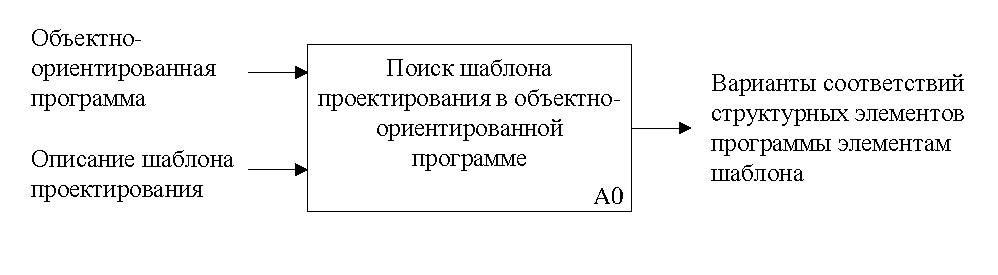
\includegraphics[width=\textwidth]{inc/idef0.pdf}
\caption{Метод поиска шаблонов проектирования в объектно-ориентированных программах}
\label{fig:idef0}
\end{figure}

\begin{figure}
\centering
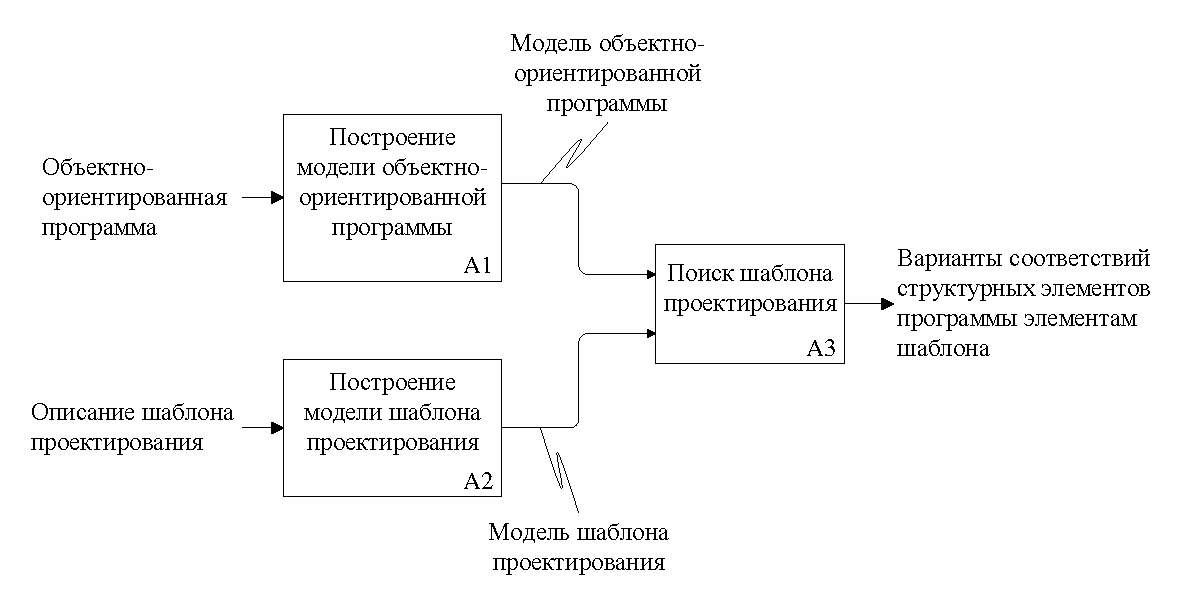
\includegraphics[width=\textwidth]{inc/idef0-general.pdf}
\caption{Метод поиска шаблонов проектирования в объектно-ориентированных программах с использованием моделей программы и шаблона}
\label{fig:idef0-general}
\end{figure}

\section{Анализ существующих методов поиска шаблонов проектирования}

Основным подходом решения поставленной задачи является сведение её к поиску
изоморфного подграфа.
Кратко рассмотрим возможные модификации такого подхода.

\subsection{Анализ метода поиска шаблонов проектирования с использованием меры схожести}

Алгоритм описан в статье <<Design Pattern Detection Using Similarity Scoring>>
~\cite{DesignPatternSimilarityScoring}.
Шаблон и программа представляются с помощю четырех ориентированных графов:
\begin{enumerate}
\item ассоциаций --- определяет ассоциации между классами;
\item обобщений --- определяет связи между базовым и производными классами;
\item абстрактных классов --- определяет, какие классы яляются абстрактными;
\item вызовов абстрактных методов --- определяет вызов из тела метода начального
класса такого же абстрактного метода другого класса.
\end{enumerate}

Графы представляются в виде матриц смежности.
Недостаток такого подхода в том, что учитываются только классы.
Отсутствие свойств и методов ведет к потере точности определения шаблонов.

Для поиска шаблонов используется алгоритм изоморфного подграфа на основе меры
схожести вершин~\cite{SimilarityGraphVertices}.
Авторы делают выбор в пользу него как неточного алгоритма исходя из следующих
преимуществ:
\begin{enumerate}
\item применимость при невозможности найти изоморфизм;
\item возможность вычисления расстояния между графами --- количества модификаций,
необходимых, чтобы один граф стал другим.
\end{enumerate}

Считается, что в контексте поиска шаблонов проектирования такой подход лучше.
Если изоморфизма не существует, не понятно действительно ли это реализация шаблона.
Возможно в реализации допущена ошибка.
Расстояние между графами может пригодиться, если нужно найти среди множества
конструкций наиболее похожую заданному шаблону.
Решение о том, является ли конструкция реализацией шаблона в этом случае является
отдельной задачей.

Точный алгоритм не используется из-за следующих недостатков:
\begin{enumerate}
\item задача является NP-полной;
\item реализация шаблона может отличаться от его описания.
\end{enumerate}

Экспоненциальное время работы может быть неприемлимо.
Описание же шаблона должно быть таким, чтобы его можно было найти в любой его
реализации. Это не может быть недостатком.

\subsection{Анализ метода поиска шаблонов проектирования на основе поиска по образцу}

Алгоритм описан в статье <<Design Pattern Detection by Template Matching>>
~\cite{DesignPatternTemplateMatching}.
В качестве модели используется набор из восьми ориентированных графов,
представленных в виде матриц смежности:
\begin{enumerate}
\item ассоциаций --- определяет ассоциации между классами;
\item обобщений --- определяет связи между базовым и производными классами;
\item абстрактных классов --- определяет, какие классы яляются абстрактными;
\item различные виды вызовов методов.
\end{enumerate}

Все матрицы смежности объединяются в одну с помощью произведения.
Предварительной каждый элемент матрицы умножается на простое число,
соответствующее этой матрице.
В итоге задача сводится к вычислению взаимнокорреляционной функции.
Матрицы при этом преобразуются в вектора.
Схожесть с шаблоном определяется косинусом угла между векторами,
считаемым специальным образом.

Этот подход более точный, чем описанный ранее за счет поиска шаблона как композиции
элементов, а не поиска отдельных составляющих.
Как и в первом случае метод применим для определения похожести,
но не для точного определения структуры системы, как композицию конструкций.

\section{Анализ существующих алгоритмов поиска изоморфных подграфов}

Задача поиска изоморфного подграфа является \textbf{NP}-полной.
Точное решение задачи в общем случае занимает экспоненциальное время.
Можно решить задачу за полиномиальное время, но с некототорой точность.
Рассмотрим соответствующие алгоритмы.

\subsection{Алгоритм поиска изоморфного подграфа на основе метода поиска в глубину}

Описан в статье <<An Algorithm for Subgraph Isomorphism>>~\cite{SubgraphIsomorphism}.
Алгоритм применим к неориентированным графам.
Находит точное решение и основан на поиске в глубину.
Графы представляются в виде матриц смежности вершин.

Изначально вершина целевого графа считается эквивалентной вершине шаблона, если
ее степень не менее степени шаблона.
Применяется процедура <<отсеивания>> лишних пар эквивалентности:
если две вершины цели связаны и каждая из них имеет эквивалентную вершину в шаблоне,
то эти две вершины шаблона должны быть связаны, иначе считается, что первая
вершина цели не имеет эквивалентных в шаблоне.
Формально условие представлено формулой~\ref{eq:ulman-equiv-condition}.

\begin{equation} \label{eq:ulman-equiv-condition}
(\forall x \in [1, p_\alpha]) ( (a_{ix} = 1) \then (\exists y \in [1, p_\beta]) (m_{xy} \cdot b_{yj} = 1) )
\end{equation}

\begin{itemize}
\item $p_\alpha$ --- количество вершин цели;
\item $p_\beta$ --- количество вершин шаблона;
\item $A = (a_{ij} \in \{ 0, 1 \})$ --- матрица смежности вершин цели;
\item $B = (b_{ij} \in \{ 0, 1 \})$ --- матрица смежности вершин шаблона;
\item $M = (m_{xy} \in \{ 0, 1 \})$ --- матрица эквивалентностей: $m_{ij} = 1$,
если вершина цели $x$ эквивалентна вершине шаблона $y$.
\end{itemize}

Точное решение единственное достоинство этого алгоритма.

К недостакам можно отмести следующее:
\begin{enumerate}
\item экспоненциальная сложность;
\item применим только к неориентированным графам;
\item не учитывает структуру вершины.
\end{enumerate}

Последние два недостатка делают алгоритм неприменимым для поставленной задачи.

\subsection{Алгоритм поиска изоморфного подграфа на основе меры схожести вершин}

Описан в статье <<A Measure Of Similarity Between Graph Vertices.
With Applications To Synonym Extraction And Web Searching>>~\cite{SimilarityGraphVertices}.
Как было показано ранее, алгоритм приводит к неточному результату.
В рамках поставленной задачи такой подход считается неприемлимым.

\section{Метод поиска шаблонов проектирования в объектно-ориентированных программах на основе поиска изоморфных подграфов}

Множество ориентированных графов --- основной вариант представления структуры
объектно-ориентированной программы.
Для программы граф можно построить сразу.
Задавать шаблон же в виде графа не удобно.
К тому же структура графов может меняться.
Нужно представление, которое можно построить для программы,
с помощью которого можно описать шаблон, и для которого можно построить необходимую
структуру графов.

UML-диаграммы классов --- один из вариантов представления структуры
объектно-ориентированной системы.
С помошью него можно описать следующие сущности:
\begin{itemize}
\item классы, интерфейсы, перечисления, примитивные типы данных;
\item свойства и методы классов;
\item связи между классами: обобщения, зависимости, ассоциации.
\end{itemize}

Шаблон проектирования также может быть описан в виде программы, специальным
формальным языком или форматом.
Такой язык или формат должен учитывать возможность неопределенности значений
некторых атрибутов элементов UML-диаграммы классов или допустимого множества.
Это необходимо, чтобы описание шаблона было более общим.

UML-диаграммы классов довольно подробно могут описывать систему.
Для описания шаблонов проектирования используется только часть элементов.
Назовем такое подмножество моделью объектно-ориентированной системы.

Итак можно выделить следующие этапы метода:
\begin{enumerate}
\item построение модели шаблона;
\item построение модели программы;
\item построение графа модели шаблона;
\item построение графа модели программы;
\item поиск изоморфного подграфа.
\end{enumerate}

Схема метода представлена на рисунке~\ref{fig:idef0-specific}.

\begin{figure}
\centering
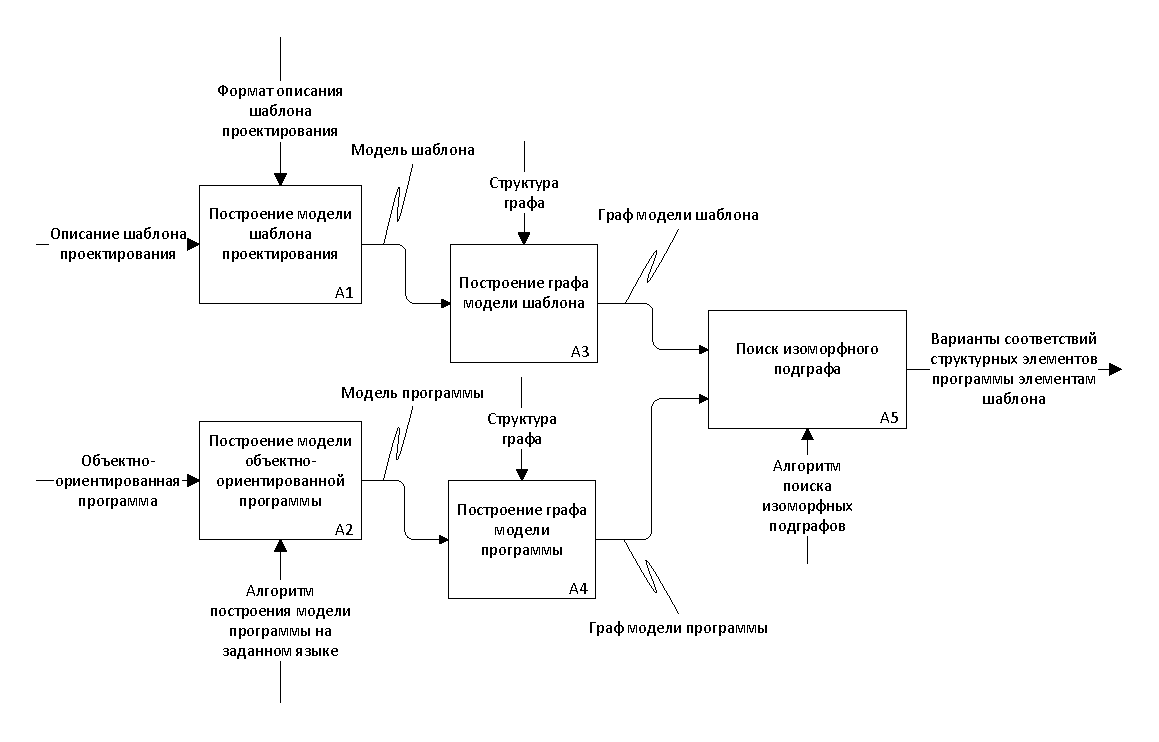
\includegraphics[angle=90]{inc/idef0-specific.pdf}
\caption{Метод поиска шаблонов проектирования в объектно-ориентированных программах на основе поиска изоморфных подграфов}
\label{fig:idef0-specific}
\end{figure}
